\newcommand{\assignmentDate}{November 18th, 2019}

% Add title
%Institute
\begin{tabular*}{\hsize}{l@{\extracolsep{\fill}} r}
	\textsc{Technical University of Berlin}		 \hfill&								 	\\
	Faculty II - Mathematics and Natural Sciences\hfill&									\\
	Institute of Mathematics 					 \hfill&									\\
	Dr. D. Peschka, A. Selahi 		 			 \hfill&									\\
\end{tabular*}

% Title
\begin{center}
	\textbf{\Large{\courseName}}\\
	\vspace{7pt}
	\large{Homework \currentAssignment}\\
	\smallskip
	\normalsize{Submitted on \assignmentDate}
\end{center}

% Group table
\begin{center}
	\vspace{-8pt}
	\begin{tabular}{l c r}
		by \textbf{\groupNumber}		    &	 			  &		 								\\
		\hline
		\texttt{Kagan Atci} 			    & \texttt{338131} & \texttt{Physical Engineering, M.Sc.}\\
		\texttt{Navneet Singh }		 	    & \texttt{380443} & \texttt{Scientific Computing, M.Sc.}\\ 
		\texttt{Daniel V. Herrmannsdoerfer} & \texttt{412543} & \texttt{Scientific Computing, M.Sc.}\\ 
		\hline
	\end{tabular}
\end{center}

% EXERCISE 1
% --------------------------------------------------------------------------------------------------------------------
\addExercise{1}{Ex1}
Considered is the Laplace operator $Lu = -\Delta$ in $\Omega = (0, L)^2$ and $u \in C^4(\bar{\Omega})$.
%
% ----------------
\newcommand{\bigO}[1]{\mathcal{O}(#1)}
\newcommand{\fixDot}{\;\cdot\;}
\addSubExercise{a}
Let $\VECT{x} = [x_1, x_2]^T \in \Omega_h$.
Applying the Laplace operator in the form of finite difference on $u(\VECT{x})$ takes place by differentiating $u(\VECT{x})$ with respect to $x_1$ and $x_2$ one at a time.
The $D^-D^+$ stencil is employed as the 2nd order finite difference operator with one neighbor on either side at the distance $h$.
\begin{align}
	\label{eq:diffX1}
	\frac{\partial^2u}{\partial x_1 ^2} = \frac{u(x_1 + h, x_2) - 2u(x_1, x_2) + u(x_1 - h, x_2)}{h^2} + \bigO{h^2}\\
	\label{eq:diffX2}
	\frac{\partial^2u}{\partial x_2 ^2} = \frac{u(x_1, x_2 + h) - 2u(x_1, x_2) + u(x_1, x_2 - h)}{h^2} + \bigO{h^2}
\end{align}
With remainders neglected in Equations (\ref{eq:diffX1}) and (\ref{eq:diffX2}), the Laplace operator can be approximated by adding both equations
\begin{equation}
	\label{eq:deltaU}
	\Delta u = \frac{u(x_1 + h, x_2) + u(x_1, x_2 + h) - 4u(x_1, x_2) + u(x_1 - h, x_2) + u(x_1, x_2 - h)}{h^2} + \bigO{h^2} \text{.}
 \end{equation}
Since $u$ is a four times continuously differentiable function in $\bar{\Omega}$ and the remainder is $\bigO{h^2}$, it holds $|| f_h -L_h R_h u||_{h} \in \bigO{h^2}$ as $h\rightarrow 0$, where $f_h$ is the right hand side of the BVP, $L_h$ the finite difference matrix and $R_h$ the restriction operator within $\bar{\Omega}$.
Hence, \EQ{deltaU}, also called as the 5-point stencil, is considered as a 2nd order consistent approximation of $\Delta u$.
%
% ----------------
\addSubExercise{b}
Unlike in the Exercise 1c of Assignment 3, a more practical way exists in building the $\MAT{L_h}$ in a sparse form using row \& column indices and the element value.
The command \texttt{sparse(ii, jj, aa)} in MATLAB serves exactly to this purpose, with \texttt{ii} and \texttt{jj} representing the vectors containing the row and column indices of the non-zero elements and \texttt{aa} the value of those elements respectively, or $L_h(ii(k),jj(k)) = aa(k)$ with $k$ being the integer in the range between 1 and the number of non-zero elements.
The key advantage of \texttt{sparse} is the handling of indices in an arbitrary sequence within the aforementioned vectors, such that the stencil coefficients can be written in lexicographically form one under the other at any arrangement.
%
% ----------------
\addSubExercise{c}
Please refer to online submitted \texttt{a04ex01\_Lh5.m} file.
%
% ----------------
\addSubExercise{d \& e}
The exercises d and e are combined in in the online submitted \texttt{a04ex01\_solve.m} file.
The function is called with a single input parameter \texttt{FLAG} that refers to the form of the numerical differentiation with
\begin{itemize}
	\item \texttt{FULL}: Solves the problem with full matrix,
	\item \texttt{RED}: Solves the problem with reduced differentiation matrix and accordingly modified right hand side.
\end{itemize}
\begin{figure}[H]
	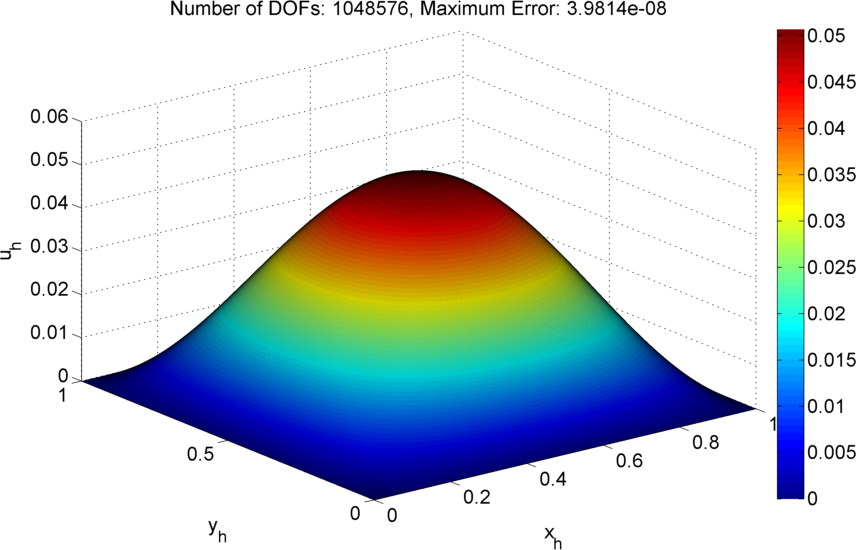
\includegraphics[width=\textwidth]{a04ex01Laplace.png} 
	\caption{Solution of $L_h u_h = \sin{(\pi x)} \sin{(\pi y)}$ with remarking the active dof number, maximum error $\max_{x,y \in \Omega_h} |u_h (x,y) - u(x,y)|$ and process duration for both flags. Since the error is same in both flags, the plot of the latter flag is omitted and the remark title is added instead.}
	\label{fig:a04ex01Laplace}
\end{figure}

The solution of $L_h u_h = \sin{(\pi x)} \sin{(\pi y)} $ with homogeneous Dirichlet boundary conditions with either differentiation forms was simulated with $512 \times 512$ points.
The result is illustrated in \FIG{a04ex01Laplace}.
It reveals that the error in both methods remain same, whereas the number of DOFs dropped significantly in the reduced method, thus nearly halving the process duration.
%
% EXERCISE 2
% --------------------------------------------------------------------------------------------------------------------
\addExercise{2}{Ex2}
%
% ----------------
\addSubExercise{a}

The right handside $f_h$ is now defined by the restriction of f to the grid points, which now can be  non uniform, and thus we can better write $f_h=f_{x}=(f(x_1),...,f(x_N))^T$. We then have to add the vector
$$
(\alpha(a\frac{2}{h_0(h_0+h_{1})}-b\frac{-1}{h_0+h_1}),0,..,0,\beta(a\frac{2}{h_{N+1}(h_N+h_{N+1})}-b\frac{1}{h_0+h_1}))^T
$$

If we use the $D^+$ stencil the middle summand of the expression of $L_h$ turns into:

$$
b(0,\frac{-1}{h_{i+1}},\frac{1}{h_{i+1}})
$$

with right hand side a sum of $f_h$ and the boundary term:

$$
(\alpha(a\frac{2}{h_0(h_0+h_{1})}),0,..,0,\beta(a\frac{2}{h_{N+1}(h_N+h_{N+1})}-b\frac{1}{h_{N+1}}))^T
$$


If we use $D^-$:

$$
b(\frac{-1}{h_{i}},\frac{1}{h_{i}},0)
$$

with right handside a sum of $f_h$ and the boundary term:

$$
(\alpha(a\frac{2}{h_0(h_0)}-b\frac{-1}{h_0+h_1}),0,..,0,\beta(a\frac{2}{h_{N+1}(h_N+h_{N+1})}))^T
$$


If we 
\addSubExercise{b}

Please refer to the online submitted \texttt{a04ex02getPDE.py} file. Figure \ref{fig:a04e02PDE_solve} shows the graph produced if the last section of the program is uncommented, which is the analytical solution from a03ex03 restricted to a uniform grid compared to the numerical solution on a uniform grid vector transformed by the function $T(x_i)=x_i^2$. We can see that the two curves are quite similar to each other, and the difference grows smaller the bigger the number of gridpoints. 

\begin{figure}[H]
	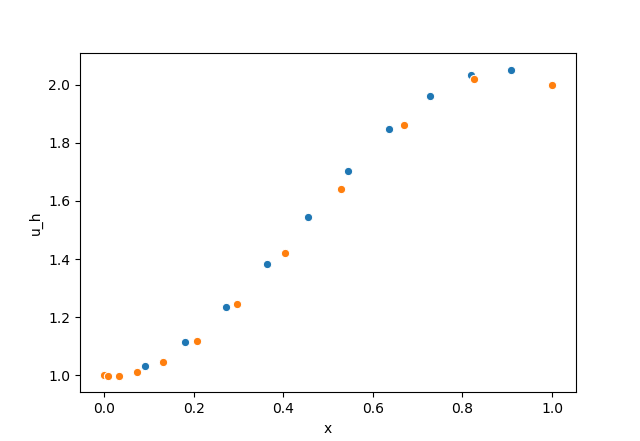
\includegraphics[width=\textwidth]{Documentation/Figures/a04ex02PDE_solved.png} 
	\caption{}
	\label{fig:a04e02PDE_solve}
\end{figure}

%
% EXERCISE 3
% --------------------------------------------------------------------------------------------------------------------
\addExercise{3}{Ex3}
%
% ----------------
\addSubExercise{a}

%
% ----------------
\addSubExercise{b}

%
% ----------------
\addSubExercise{c}

%
% ----------------
\addSubExercise{d}